\documentclass[10pt,a4paper]{article}
\usepackage[margin=2cm]{geometry}
\usepackage{amsmath,amssymb}
\usepackage{booktabs,array,longtable}
\usepackage{graphicx}
\usepackage{float}
\usepackage[font=small,labelfont=bf,skip=4pt]{caption}
\usepackage{xcolor}
\usepackage[hidelinks]{hyperref}
\renewcommand{\thetable}{S\arabic{table}}
\renewcommand{\thefigure}{S\arabic{figure}}
\newcommand{\cfg}[1]{\texttt{#1}}
\setlength{\parindent}{0pt}\setlength{\parskip}{4pt}

\begin{document}

{\large\bfseries Additional file 1: Supplementary results}\par
\smallskip
Evidence before prediction: a configuration-driven framework for testing how molecular descriptors shape property models\par
\medskip

\textbf{Abbreviations.} AP, average precision; AUROC, area under the receiver operating characteristic curve; BBBP, blood-brain barrier penetration; BACE-1, beta-site amyloid precursor protein cleaving enzyme 1; BCE, binary cross-entropy; CI, confidence interval; D-MPNN, directed message-passing neural network; ECFP4, extended-connectivity fingerprint with radius 2; ESOL, the aqueous-solubility benchmark; FFN, feed-forward network; GIN, graph isomorphism network; InChIKey, International Chemical Identifier key; L1, absolute-value regularisation; LARS, least angle regression; MAE, mean absolute error; MI, mutual information; MI--Pearson, mutual-information relevance with Pearson-correlation redundancy; MLP, multilayer perceptron; OOD, out of distribution, used here as a range-based descriptor diagnostic; RF, Random Forest; RMSE, root mean squared error; SD, standard deviation; SMILES, simplified molecular input line entry system; TDC, Therapeutics Data Commons.

\textbf{Contents.} Dataset overview, source-level target statistics, and provenance (Table~\ref{tab:dataset-summary}); fixed hyperparameters (Table~\ref{tab:hp}); scorecard diagnostics (Table~\ref{tab:shift}); recommended versus random subsets and the full pool (Table~\ref{tab:rec-random}); six-selector results and stability (Table~\ref{tab:sel-full}, Fig.~\ref{fig:selectors}) and the selector comparisons that survive multiplicity correction (Table~\ref{tab:selector-stats}); internal and external paired comparisons (Tables~\ref{tab:int}--\ref{tab:ext}); harmonised descriptor-routing results and their paired comparisons (Tables~\ref{tab:routing-si} and \ref{tab:routing-stats}); training-seed variance (Table~\ref{tab:seed}); secondary metrics (Table~\ref{tab:secondary}); per-split primary scores (Table~\ref{tab:splits}); Caco-2 advisor case study (Table~\ref{tab:caco2}); duplicate-controlled BBBP sensitivity analysis and its paired comparisons (Tables~\ref{tab:bbbp-sensitivity} and \ref{tab:bbbp-sensitivity-stats}); checkpoint protocol and result-file inventory (Table~\ref{tab:routing-audit}).

\textbf{Conventions.} Unless stated otherwise, scores are measured on the test partition of the ten saved split manifests, with split $s=1,\dots,10$ corresponding to seed $s$. The duplicate controlled BBBP sensitivity analysis uses new manifests described in Table~\ref{tab:bbbp-sensitivity}. Means are reported with population standard deviation (SD). Root mean squared error (RMSE) is better when lower; area under the receiver operating characteristic curve (AUROC) is better when higher. Paired differences are $\Delta_s=m_A(s)-m_B(s)$, and wins count the splits on which $A$ is better. The descriptive 95\% confidence interval uses $\bar\Delta\pm t_{0.975,9}\,s_\Delta/\sqrt{10}$, where $s_\Delta$ is the sample standard deviation of the paired differences; because training sets overlap, the corrected Nadeau--Bengio intervals in Tables~\ref{tab:int}--\ref{tab:ext} and \ref{tab:routing-stats} inflate the variance by $1/k+n_{\mathrm{test}}/n_{\mathrm{train}}$ and are the intervals used for inference. Tables were generated from result files written by scripts in \texttt{benchmarks/} of the repository.

% ---------------------------------------------------------------------------
\section*{Dataset overview and provenance}

\renewcommand{\thetable}{S1a}
\begin{table}[H]
\caption{Dataset overview, target definitions, source-level target distributions, and provenance. $N$ is the number of records retained for this study after the stated preprocessing. Published target summaries are shown for the original dataset release and are not recomputed from the individual train, validation, or test partitions.}\label{tab:dataset-summary}
\centering\footnotesize
\setlength{\tabcolsep}{2pt}
\begin{tabular}{@{}>{\raggedright\arraybackslash}p{0.10\textwidth}>{\raggedright\arraybackslash}p{0.20\textwidth}>{\raggedright\arraybackslash}p{0.27\textwidth}>{\raggedright\arraybackslash}p{0.12\textwidth}>{\raggedright\arraybackslash}p{0.08\textwidth}>{\raggedright\arraybackslash}p{0.15\textwidth}@{}}
\toprule
Dataset ($N$ used) & Target / output & Source-level target distribution & Task / metric & Split & Original source \\
\midrule
ESOL (1,128) & Measured aqueous solubility, $\log_{10}$ mol L$^{-1}$ & Mean $-3.05$; SD $2.10$; range $[-11.60,1.58]$ & Regression; RMSE & Scaffold & Delaney (2004) \\
FreeSolv (642) & Experimental hydration free energy, kcal mol$^{-1}$ & Mean $-3.80$; SD $3.85$; range $[-25.47,3.43]$ & Regression; RMSE & Random & Mobley et al. (2014); FreeSolv v0.52 \\
Lipophilicity (4,200) & Octanol/water distribution coefficient, $\log D$ at pH 7.4 & Mean $2.19$; SD $1.20$; assay range $[-1.5,4.5]$ & Regression; RMSE & Scaffold & Hersey et al. / ChEMBL (2015) \\
BBBP (2,039) & Blood--brain barrier permeability label & Original file: 1,567 positive (76.4\%) and 483 negative of 2,050; 11 unparseable SMILES removed & Binary classification; AUROC & Scaffold & Martins et al. (2012) \\
BACE (1,513) & BACE-1 inhibitor/activity label & 691 positive/active (45.7\%) and 822 negative/inactive (54.3\%) & Binary classification; AUROC & Scaffold & Subramanian et al. (2016) \\
\bottomrule
\end{tabular}
\end{table}

The target summaries above are included to contextualise the prediction problems, not as evidence calculated from held-out labels. The counts used in the model benchmark follow the processed data described in the manuscript. In particular, the BBBP source release contains 2,050 records, whereas the primary benchmark contains 2,039 because 11 SMILES could not be parsed by RDKit. In the duplicate-controlled BBBP sensitivity analysis, the data composition and split manifests change again; those counts and class totals are reported separately in Table~\ref{tab:bbbp-sensitivity}.

% ---------------------------------------------------------------------------
\section*{Hyperparameters}

\renewcommand{\thetable}{S1b}

\begin{table}[H]
\caption{Fixed hyperparameters. No hyperparameter was tuned on test data; $K^*$ in the routing experiment was the only quantity selected, on validation.}\label{tab:hp}
\centering\footnotesize
\begin{tabular}{@{}>{\raggedright\arraybackslash}p{0.27\textwidth}>{\raggedright\arraybackslash}p{0.68\textwidth}@{}}
\toprule
Model & Settings \\
\midrule
ECFP4 + Random Forest & Morgan fingerprint, radius 2, 2,048 bits; 100 trees, scikit-learn defaults otherwise \\
RDKit 2D + Random Forest & 210 RDKit 2D descriptors (RDKit 2023.09.6), non-finite values set to 0; 100 trees \\
Descriptor MLP (reference) & 210 $\rightarrow$ 128 $\rightarrow$ 64 $\rightarrow$ 1, LayerNorm, dropout 0.2; AdamW (lr $10^{-3}$, weight decay $10^{-4}$), batch 64, 50 epochs, Huber or BCE-with-logits loss, checkpoint on validation loss \\
Framework role ablation (\cfg{direct\_only}, \cfg{residual\_only}, \cfg{direct\_hybrid}, \cfg{prior\_residual}) & D-MPNN, hidden 128, depth 3, sum aggregation; descriptor encoder 210 $\rightarrow$ 64 with LayerNorm; head 192 $\rightarrow$ 64 $\rightarrow$ 1; dropout 0.2; AdamW (lr $10^{-3}$, weight decay $10^{-4}$), batch 64, 40 epochs, checkpoint on validation loss; standard scaling fitted on training data \\
Prior (\cfg{prior\_only}, \cfg{prior\_residual}) & Six descriptors (MolWt, MolLogP, TPSA, NumHDonors, NumHAcceptors, NumRotatableBonds); ridge regression ($\alpha=1$) or logistic regression ($C=1$, log-odds from \cfg{decision\_function}), fitted on training data and frozen \\
Harmonised routing experiment & Same architecture and optimiser as the role ablation; $K\in\{10,20,50\}$; all route checkpoints selected by minimum validation loss; $K^*$ selected using the primary validation metric at that checkpoint; random routes averaged over ten draws per split \\
Checkpoint audit & Completed across five datasets; 250 model runs logged in \url{routing_checkpoint_audit.csv}; dataset-level outputs are listed in Table~\ref{tab:routing-audit} \\
Chemprop v2.3.1 & Bond message passing, hidden size 300, depth 3, dropout 0, mean aggregation, batch normalisation; FFN with one hidden layer of 300; default learning-rate schedule; batch 64; up to 50 epochs, early stopping on validation loss (patience 10); target and descriptor scaling fitted on training data \\
Selector comparison & MI: $k=3$ neighbours; MI--Pearson: MI relevance minus mean $|$Pearson$|$ redundancy; RF importance: 100 trees, max depth 12; L1: LARS--lasso entry order (regression) or $|$coefficient$|$ of L1-logistic regression, $C=1$ (classification); L1 feature scaling fitted on training data only; downstream Random Forest with 100 trees \\
\bottomrule
\end{tabular}
\end{table}
\setcounter{table}{1}
\renewcommand{\thetable}{S\arabic{table}}

% ---------------------------------------------------------------------------
\section*{Scorecard diagnostics}

\begin{table}[H]
\caption{Range-based covariate shift. (a) Illustrative scaffold split 1 versus a random 80/10/10 split of the same data. OOD descriptors: descriptors with any test value outside the training range. Evidence classes in this case study follow a simplified rule of the audit script: out-of-range or zero training support $\rightarrow$ OOD/unsupported; $|r|>0.85$ with an earlier feature $\rightarrow$ redundant; training $|\rho_{\mathrm{Spearman}}|\geq0.15$ $\rightarrow$ supported; otherwise weak. (b) The ten BBBP scaffold splits with the number of out-of-range descriptors, the number of test molecules affected, and the test AUROC of four role-ablation models.}\label{tab:shift}
\centering\footnotesize
\textbf{(a)}\par\smallskip
\begin{tabular}{@{}llrrrrrr@{}}
\toprule
Dataset & Split & OOD descriptors & Test molecules affected & OOD/unsupported & Redundant & Supported & Weak \\
\midrule
ESOL & Scaffold & 20 (9.5\%) & 7.1\% & 39 & 48 & 34 & 89 \\
 & Random & 8 (3.8\%) & 5.3\% & 27 & 51 & 35 & 97 \\
Lipophilicity & Scaffold & 11 (5.2\%) & 3.1\% & 21 & 43 & 25 & 121 \\
 & Random & 7 (3.3\%) & 1.7\% & 17 & 45 & 23 & 125 \\
\bottomrule
\end{tabular}

\medskip\textbf{(b)}\par\smallskip
\begin{tabular}{@{}lrrcccc@{}}
\toprule
Split & OOD descriptors & Test molecules affected & \cfg{direct\_only} & \cfg{direct\_hybrid} & \cfg{residual\_only} & \cfg{prior\_residual} \\
\midrule
1 & 34 (16.2\%) & 10 (4.9\%) & 0.9320 & 0.9367 & 0.9162 & 0.9375 \\
2 & 5 (2.4\%) & 4 (2.0\%) & 0.8721 & 0.9118 & 0.8265 & 0.8277 \\
3 & 18 (8.6\%) & 7 (3.4\%) & 0.9429 & 0.9507 & 0.9270 & 0.9291 \\
4 & 8 (3.8\%) & 9 (4.4\%) & 0.9214 & 0.9110 & 0.9243 & 0.9108 \\
5 & 12 (5.7\%) & 5 (2.5\%) & 0.8819 & 0.8958 & 0.9386 & 0.9331 \\
6 & 16 (7.6\%) & 11 (5.4\%) & 0.8174 & 0.8833 & 0.8850 & 0.9109 \\
7 & 4 (1.9\%) & 5 (2.5\%) & 0.9496 & 0.9659 & 0.9496 & 0.9455 \\
8 & 19 (9.0\%) & 18 (8.8\%) & 0.8578 & 0.8671 & 0.9413 & 0.9302 \\
9 & 6 (2.9\%) & 4 (2.0\%) & 0.9319 & 0.9280 & 0.9258 & 0.8854 \\
10 & 28 (13.3\%) & 3 (1.5\%) & 0.9240 & 0.9115 & 0.9097 & 0.8872 \\
\bottomrule
\end{tabular}
\end{table}

Across all ten scaffold splits, the mean number of out-of-range descriptors was $19.4\pm12.8$ for ESOL ($9.2\pm6.1\%$ of the 210 descriptors), $20.8\pm14.8$ for Lipophilicity ($9.9\pm7.1\%$), and $15.1\pm9.5$ for BBBP ($7.2\pm4.5\%$). The mean fraction of test molecules affected was $6.3\pm2.5\%$, $3.7\pm0.7\%$, and $3.8\pm2.1\%$, respectively. The scaffold-versus-random values in Table~\ref{tab:shift}(a) are a split-1 illustration, not averages across split manifests.

% ---------------------------------------------------------------------------
\section*{Recommended subsets versus random subsets and the full pool}

\begin{table}[H]
\caption{Framework-recommended top-$K$ subsets versus random $K$-subsets (ten draws per split, averaged) and versus the full 210-descriptor pool, with a Random Forest downstream. All entries are paired on the same 10 splits. $\bar\Delta$ is the mean paired difference, recommended minus the comparator, so a negative value in panel (a) and a positive value in panel (b) mean that the recommended subset scores worse than the comparator (RMSE for ESOL and FreeSolv; AUROC for BBBP). $p_{\mathrm{H}}$ is Holm-adjusted within each dataset across the eight comparisons of the two panels ($m=8$); $^{*}p_{\mathrm{H}}<0.05$, $^{**}p_{\mathrm{H}}<0.01$. Against random subsets of the same size, the recommended subsets score significantly better at ESOL $K=5$, ESOL $K=10$, ESOL $K=20$, ESOL $K=50$, FreeSolv $K=5$, FreeSolv $K=10$, FreeSolv $K=20$, and BBBP $K=5$ and nowhere worse; the remaining 4 of the 12 dataset-budget cells do not separate. Against the full 210-descriptor pool, the recommended subsets are significantly worse at ESOL $K=5$ and ESOL $K=10$, and no other cell separates (10 of 12 cells inconclusive). Random subsets average ten draws per split, so differences against them carry the draw noise of the comparator. Contrast this table with the corresponding rows of Table~\ref{tab:routing-si}, where the same recommendation is routed into a graph hybrid rather than used directly; the two experiments ask different questions and are not expected to agree.}\label{tab:rec-random}
\centering\scriptsize
\setlength{\tabcolsep}{4pt}
\textbf{(a) Recommended versus random subsets}\par\smallskip
\begin{tabular}{@{}llcccc@{}}
\toprule
Dataset & $K$ & $\bar\Delta$ & Corrected 95\% interval & $p_{\mathrm{H}}$ & Wins of recommended \\
\midrule
ESOL & 5 & $-0.745$ & $[-0.894,-0.596]$ & $<0.001^{**}$ & 10/10 \\
 & 10 & $-0.419$ & $[-0.526,-0.313]$ & $<0.001^{**}$ & 10/10 \\
 & 20 & $-0.204$ & $[-0.307,-0.102]$ & $0.006^{**}$ & 10/10 \\
 & 50 & $-0.116$ & $[-0.165,-0.068]$ & $0.002^{**}$ & 10/10 \\
\midrule
FreeSolv & 5 & $-1.546$ & $[-1.924,-1.169]$ & $<0.001^{**}$ & 10/10 \\
 & 10 & $-1.009$ & $[-1.223,-0.794]$ & $<0.001^{**}$ & 10/10 \\
 & 20 & $-0.567$ & $[-0.785,-0.350]$ & $0.001^{**}$ & 10/10 \\
 & 50 & $-0.300$ & $[-0.515,-0.084]$ & $0.059$ & 10/10 \\
\midrule
BBBP & 5 & $+0.096$ & $[0.039,0.152]$ & $0.032^{*}$ & 10/10 \\
 & 10 & $+0.043$ & $[0.007,0.078]$ & $0.140$ & 8/10 \\
 & 20 & $+0.015$ & $[-0.006,0.036]$ & $0.551$ & 8/10 \\
 & 50 & $+0.004$ & $[-0.005,0.014]$ & $0.671$ & 4/10 \\
\bottomrule
\end{tabular}

\medskip\textbf{(b) Recommended versus the full 210-descriptor pool}\par\smallskip
\begin{tabular}{@{}llcccc@{}}
\toprule
Dataset & $K$ & $\bar\Delta$ & Corrected 95\% interval & $p_{\mathrm{H}}$ & Wins of recommended \\
\midrule
ESOL & 5 & $+0.063$ & $[0.031,0.094]$ & $0.006^{**}$ & 0/10 \\
 & 10 & $+0.080$ & $[0.048,0.111]$ & $0.002^{**}$ & 0/10 \\
 & 20 & $+0.055$ & $[0.002,0.107]$ & $0.088$ & 0/10 \\
 & 50 & $+0.010$ & $[-0.016,0.036]$ & $0.389$ & 5/10 \\
\midrule
FreeSolv & 5 & $+0.321$ & $[0.062,0.580]$ & $0.082$ & 1/10 \\
 & 10 & $+0.151$ & $[-0.022,0.324]$ & $0.238$ & 2/10 \\
 & 20 & $+0.092$ & $[-0.042,0.227]$ & $0.310$ & 2/10 \\
 & 50 & $-0.019$ & $[-0.097,0.058]$ & $0.584$ & 5/10 \\
\midrule
BBBP & 5 & $-0.048$ & $[-0.084,-0.012]$ & $0.097$ & 1/10 \\
 & 10 & $-0.023$ & $[-0.050,0.003]$ & $0.376$ & 2/10 \\
 & 20 & $-0.009$ & $[-0.023,0.006]$ & $0.629$ & 2/10 \\
 & 50 & $-0.001$ & $[-0.010,0.007]$ & $0.766$ & 3/10 \\
\bottomrule
\end{tabular}
\end{table}

% ---------------------------------------------------------------------------
\section*{Six feature selectors}

\begin{table}[H]
\caption{Six feature selectors with a Random Forest downstream, on the ten saved splits. (a) Mean test score per selector and budget (RMSE for ESOL, FreeSolv and Lipophilicity, AUROC for BBBP and BACE); bold marks the best mean within each dataset and budget. (b) Mean pairwise Jaccard index of the selected sets across splits, averaged over $K\in\{5,10,20,50\}$. The selector previously labelled mRMR is named MI--Pearson here because its redundancy term is mean absolute Pearson correlation rather than mutual information. The table reports selectors as the learner's only input; Table~\ref{tab:routing-si} instead routes the recommended subset into a graph hybrid.}\label{tab:sel-full}
\centering\scriptsize
\setlength{\tabcolsep}{4pt}
% (a) per-budget means
\textbf{(a) Test score by selector and budget}\par\smallskip
\begin{tabular}{@{}llcccc@{}}
\toprule
Dataset (metric) & Selector & $K=5$ & $K=10$ & $K=20$ & $K=50$ \\
\midrule
ESOL (RMSE $\downarrow$) & Framework recommender & $0.700$ & $0.716$ & $0.692$ & $0.647$ \\
 & L1 (lasso / L1-logistic) & $0.734$ & $0.729$ & $0.704$ & $0.675$ \\
 & MI--Pearson & $0.711$ & $0.677$ & $0.658$ & $0.659$ \\
 & Mutual information & $0.682$ & $0.661$ & $0.663$ & $0.651$ \\
 & RF impurity importance & $\mathbf{0.678}$ & $\mathbf{0.633}$ & $\mathbf{0.640}$ & $\mathbf{0.640}$ \\
 & Spearman top-$K$ & $0.718$ & $0.668$ & $0.664$ & $0.648$ \\
\midrule
FreeSolv (RMSE $\downarrow$) & Framework recommender & $1.410$ & $1.240$ & $1.182$ & $\mathbf{1.070}$ \\
 & L1 (lasso / L1-logistic) & $1.724$ & $1.350$ & $1.245$ & $1.229$ \\
 & MI--Pearson & $1.281$ & $1.263$ & $1.183$ & $1.106$ \\
 & Mutual information & $\mathbf{1.243}$ & $1.192$ & $1.168$ & $1.124$ \\
 & RF impurity importance & $1.277$ & $\mathbf{1.108}$ & $\mathbf{1.095}$ & $1.077$ \\
 & Spearman top-$K$ & $1.456$ & $1.222$ & $1.170$ & $1.074$ \\
\midrule
Lipophilicity (RMSE $\downarrow$) & Framework recommender & $0.941$ & $0.850$ & $0.788$ & $0.768$ \\
 & L1 (lasso / L1-logistic) & $0.964$ & $0.905$ & $0.821$ & $0.784$ \\
 & MI--Pearson & $0.880$ & $0.831$ & $0.800$ & $0.779$ \\
 & Mutual information & $\mathbf{0.857}$ & $\mathbf{0.814}$ & $0.783$ & $0.763$ \\
 & RF impurity importance & $0.922$ & $0.822$ & $\mathbf{0.780}$ & $\mathbf{0.759}$ \\
 & Spearman top-$K$ & $0.984$ & $0.857$ & $0.798$ & $0.782$ \\
\midrule
BBBP (AUROC $\uparrow$) & Framework recommender & $0.864$ & $0.889$ & $0.904$ & $0.911$ \\
 & L1 (lasso / L1-logistic) & $0.832$ & $0.891$ & $0.906$ & $\mathbf{0.919}$ \\
 & MI--Pearson & $\mathbf{0.884}$ & $\mathbf{0.906}$ & $\mathbf{0.912}$ & $0.914$ \\
 & Mutual information & $0.879$ & $0.899$ & $0.904$ & $0.916$ \\
 & RF impurity importance & $0.860$ & $0.886$ & $0.903$ & $0.909$ \\
 & Spearman top-$K$ & $0.853$ & $0.875$ & $0.899$ & $0.907$ \\
\midrule
BACE (AUROC $\uparrow$) & Framework recommender & $0.758$ & $0.780$ & $0.796$ & $0.818$ \\
 & L1 (lasso / L1-logistic) & $0.716$ & $0.764$ & $0.797$ & $\mathbf{0.820}$ \\
 & MI--Pearson & $\mathbf{0.786}$ & $0.793$ & $0.808$ & $0.807$ \\
 & Mutual information & $0.783$ & $0.793$ & $0.807$ & $0.809$ \\
 & RF impurity importance & $0.773$ & $\mathbf{0.796}$ & $\mathbf{0.810}$ & $0.818$ \\
 & Spearman top-$K$ & $0.748$ & $0.763$ & $0.772$ & $0.798$ \\
\bottomrule
\end{tabular}

\medskip\textbf{(b) Mean pairwise Jaccard stability across splits}\par\smallskip
\begin{tabular}{@{}lccccc@{}}
\toprule
Selector & ESOL & FreeSolv & Lipophilicity & BBBP & BACE \\
\midrule
Framework recommender & 0.78 & 0.84 & 0.79 & 0.76 & 0.62 \\
L1 (lasso / L1-logistic) & 0.50 & 0.38 & 0.59 & 0.51 & 0.39 \\
MI--Pearson & 0.56 & 0.78 & 0.43 & 0.46 & 0.61 \\
Mutual information & 0.86 & 0.88 & 0.63 & 0.82 & 0.83 \\
RF impurity importance & 0.67 & 0.71 & 0.70 & 0.62 & 0.57 \\
Spearman top-$K$ & 0.96 & 0.92 & 0.82 & 0.85 & 0.86 \\
\bottomrule
\end{tabular}
\end{table}

\renewcommand{\thetable}{S4b}
\begin{table}[H]
\caption{Selector comparisons that survive Holm correction within a dataset (family $m=20$: the five other selectors against the framework selector at four budgets, on the same ten splits as Table~\ref{tab:sel-full}). Of the 100 selector comparisons, 2 survive: \texttt{rf\_importance} $K=10$ vs framework $K=10$ on ESOL and mutual\_information $K=5$ vs framework $K=5$ on Lipophilicity. On the other endpoints no selector separates from the framework selector once multiplicity is controlled, which is consistent with the mean-rank table rather than in tension with it.}\label{tab:selector-stats}
\centering\scriptsize
\setlength{\tabcolsep}{4pt}
\begin{tabular}{@{}llccccr@{}}
\toprule
Dataset & Comparison ($A$ vs $B$) & $\bar\Delta\pm\mathrm{SD}$ & Corrected 95\% interval & $p$ & $p_{\mathrm{H}}$ & Wins of $A$ \\
\midrule
ESOL & \texttt{rf\_importance} $K=10$ vs framework $K=10$ & $-0.084\pm0.034$ & $[-0.122,-0.046]$ & $<0.001$ & $0.015^{*}$ & 10/10 \\
FreeSolv & \multicolumn{6}{l}{no comparison survives the correction} \\
Lipophilicity & mutual\_information $K=5$ vs framework $K=5$ & $-0.084\pm0.025$ & $[-0.113,-0.055]$ & $<0.001$ & $0.002^{**}$ & 10/10 \\
BBBP & \multicolumn{6}{l}{no comparison survives the correction} \\
BACE & \multicolumn{6}{l}{no comparison survives the correction} \\
\bottomrule
\end{tabular}
\end{table}
\addtocounter{table}{-1}
\renewcommand{\thetable}{S\arabic{table}}

\begin{figure}[H]
\centering
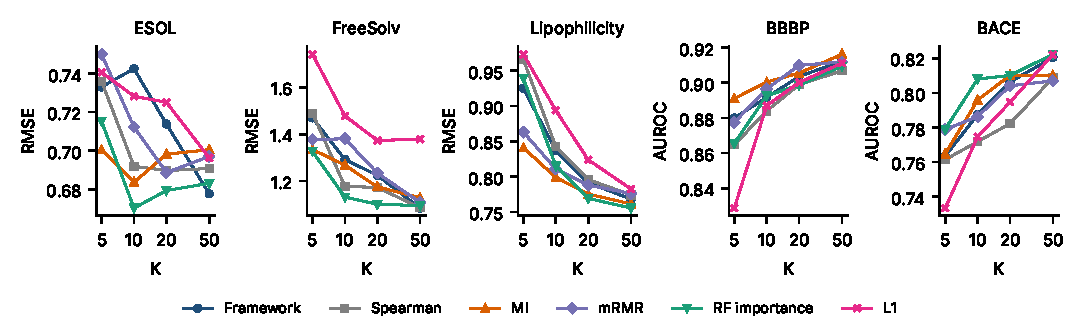
\includegraphics[width=\textwidth]{figS1_selectors.pdf}
\caption{Mean test score of the six selectors as a function of the descriptor budget $K$ (Random Forest downstream). Lower is better for RMSE, higher for AUROC. The former mRMR implementation is labelled MI--Pearson.}\label{fig:selectors}
\end{figure}

% ---------------------------------------------------------------------------
\section*{Paired comparisons}

\begin{table}[H]
\caption{Internal paired comparisons on the main models. Hybrid: \cfg{direct\_hybrid}; graph only: \cfg{residual\_only}; prior/residual: \cfg{prior\_residual}. All entries are paired on the same 10 saved splits, and win counts are out of 10. $\bar\Delta$ is the mean paired difference $m_A-m_B$ with the population SD of the differences; wins count the splits on which $A$ was better. Both intervals are two-sided $t$ intervals with 9 degrees of freedom: the nominal interval uses the paired standard error, and the corrected interval inflates the variance by $1/k+n_{\mathrm{test}}/n_{\mathrm{train}}$ to reflect the overlap of the training partitions (Nadeau--Bengio). $p$ is the corrected two-sided $p$-value and $p_{\mathrm{H}}$ is Holm-adjusted within this table ($m=20$); $^{*}p_{\mathrm{H}}<0.05$, $^{**}p_{\mathrm{H}}<0.01$. The comparisons that survive Holm correction are Hybrid vs RDKit 2D + RF on Lipophilicity and Hybrid vs RDKit 2D + RF on BACE; every other entry is reported as inconclusive. }\label{tab:int}
\centering\scriptsize
\setlength{\tabcolsep}{4pt}
\resizebox{\textwidth}{!}{%
\begin{tabular}{@{}llccccccc@{}}
\toprule
Dataset (metric) & Comparison ($A$ vs $B$) & $\bar\Delta\pm\mathrm{SD}$ & Nominal 95\% interval & Corrected 95\% interval & $p$ & $p_{\mathrm{H}}$ & Wins of $A$ \\
\midrule
ESOL (RMSE) & Hybrid vs RDKit 2D + RF & $-0.014\pm0.0622$ & $[-0.061,0.033]$ & $[-0.085,0.056]$ & $0.657$ & $1.000$ & 5/10 \\
 & Hybrid vs Graph only & $-0.001\pm0.0844$ & $[-0.064,0.063]$ & $[-0.096,0.095]$ & $0.986$ & $1.000$ & 7/10 \\
 & Prior/residual vs Graph only & $+0.057\pm0.0990$ & $[-0.018,0.132]$ & $[-0.055,0.169]$ & $0.278$ & $0.899$ & 4/10 \\
 & Prior/residual vs Hybrid & $+0.058\pm0.0888$ & $[-0.009,0.125]$ & $[-0.043,0.158]$ & $0.225$ & $0.899$ & 2/10 \\
\midrule
FreeSolv (RMSE) & Hybrid vs RDKit 2D + RF & $+0.010\pm0.1737$ & $[-0.121,0.141]$ & $[-0.187,0.207]$ & $0.913$ & $1.000$ & 5/10 \\
 & Hybrid vs Graph only & $-0.152\pm0.2523$ & $[-0.342,0.039]$ & $[-0.438,0.135]$ & $0.262$ & $1.000$ & 6/10 \\
 & Prior/residual vs Graph only & $-0.076\pm0.2818$ & $[-0.288,0.137]$ & $[-0.396,0.244]$ & $0.605$ & $1.000$ & 7/10 \\
 & Prior/residual vs Hybrid & $+0.076\pm0.3086$ & $[-0.157,0.309]$ & $[-0.275,0.426]$ & $0.636$ & $1.000$ & 4/10 \\
\midrule
Lipophilicity (RMSE) & Hybrid vs RDKit 2D + RF & $-0.142\pm0.0323$ & $[-0.167,-0.118]$ & $[-0.179,-0.106]$ & $<0.001$ & $<0.001^{**}$ & 10/10 \\
 & Hybrid vs Graph only & $-0.001\pm0.0228$ & $[-0.018,0.016]$ & $[-0.027,0.025]$ & $0.943$ & $1.000$ & 5/10 \\
 & Prior/residual vs Graph only & $+0.002\pm0.0332$ & $[-0.023,0.028]$ & $[-0.035,0.040]$ & $0.885$ & $1.000$ & 6/10 \\
 & Prior/residual vs Hybrid & $+0.003\pm0.0285$ & $[-0.018,0.025]$ & $[-0.029,0.036]$ & $0.821$ & $1.000$ & 6/10 \\
\midrule
BBBP (AUROC) & Hybrid vs RDKit 2D + RF & $+0.004\pm0.0283$ & $[-0.017,0.025]$ & $[-0.028,0.036]$ & $0.783$ & $1.000$ & 5/10 \\
 & Hybrid vs Graph only & $+0.002\pm0.0400$ & $[-0.028,0.032]$ & $[-0.043,0.047]$ & $0.931$ & $1.000$ & 6/10 \\
 & Prior/residual vs Graph only & $-0.005\pm0.0184$ & $[-0.019,0.009]$ & $[-0.026,0.016]$ & $0.625$ & $1.000$ & 4/10 \\
 & Prior/residual vs Hybrid & $-0.006\pm0.0401$ & $[-0.037,0.024]$ & $[-0.052,0.039]$ & $0.755$ & $1.000$ & 4/10 \\
\midrule
BACE (AUROC) & Hybrid vs RDKit 2D + RF & $-0.037\pm0.0182$ & $[-0.051,-0.023]$ & $[-0.058,-0.017]$ & $0.003$ & $0.011^{*}$ & 0/10 \\
 & Hybrid vs Graph only & $-0.017\pm0.0357$ & $[-0.044,0.010]$ & $[-0.057,0.024]$ & $0.368$ & $1.000$ & 2/10 \\
 & Prior/residual vs Graph only & $-0.019\pm0.0495$ & $[-0.057,0.018]$ & $[-0.075,0.037]$ & $0.457$ & $1.000$ & 4/10 \\
 & Prior/residual vs Hybrid & $-0.002\pm0.0478$ & $[-0.038,0.034]$ & $[-0.057,0.052]$ & $0.924$ & $1.000$ & 6/10 \\
\bottomrule
\end{tabular}
}
\end{table}

\begin{table}[H]
\caption{Framework minus Chemprop v2.3.1 on matched splits, for the graph only model and for the graph model with the 210 descriptors. Conventions follow Table~\ref{tab:int}; all entries are paired on the same 10 splits and $p_{\mathrm{H}}$ is Holm-adjusted within this table ($m=10$). No comparison in this table survives Holm correction, so every entry is reported as inconclusive. Adding the 210 descriptors raises the mean score in both implementations on FreeSolv, Lipophilicity, and BBBP, lowers it in both on BACE, and disagrees between implementations on ESOL. Because a comparison between the two implementations at this sample size is underpowered, the agreement is descriptive.}\label{tab:ext}
\centering\scriptsize
\setlength{\tabcolsep}{4pt}
\resizebox{\textwidth}{!}{%
\begin{tabular}{@{}llcccccc@{}}
\toprule
Dataset (metric) & Model pair & $\bar\Delta\pm\mathrm{SD}$ & Nominal 95\% interval & Corrected 95\% interval & $p$ & $p_{\mathrm{H}}$ & Wins of framework \\
\midrule
ESOL (RMSE) & graph only & $-0.167\pm0.1261$ & $[-0.262,-0.072]$ & $[-0.310,-0.024]$ & $0.026$ & $0.053$ & 9/10 \\
ESOL (RMSE) & graph + 210 descriptors & $-0.221\pm0.6143$ & $[-0.685,0.242]$ & $[-0.917,0.474]$ & $0.490$ & $0.490$ & 7/10 \\
FreeSolv (RMSE) & graph only & $+0.073\pm0.2786$ & $[-0.137,0.283]$ & $[-0.243,0.389]$ & $0.615$ & $0.615$ & 3/10 \\
FreeSolv (RMSE) & graph + 210 descriptors & $+0.153\pm0.1913$ & $[0.009,0.298]$ & $[-0.064,0.370]$ & $0.145$ & $0.290$ & 1/10 \\
Lipophilicity (RMSE) & graph only & $-0.034\pm0.0775$ & $[-0.092,0.025]$ & $[-0.121,0.054]$ & $0.408$ & $0.581$ & 7/10 \\
Lipophilicity (RMSE) & graph + 210 descriptors & $-0.033\pm0.0593$ & $[-0.078,0.011]$ & $[-0.100,0.034]$ & $0.290$ & $0.581$ & 6/10 \\
BBBP (AUROC) & graph only & $+0.003\pm0.0378$ & $[-0.025,0.032]$ & $[-0.039,0.046]$ & $0.859$ & $1.000$ & 4/10 \\
BBBP (AUROC) & graph + 210 descriptors & $-0.007\pm0.0209$ & $[-0.023,0.009]$ & $[-0.031,0.017]$ & $0.529$ & $1.000$ & 5/10 \\
BACE (AUROC) & graph only & $-0.006\pm0.0294$ & $[-0.028,0.017]$ & $[-0.039,0.028]$ & $0.710$ & $1.000$ & 3/10 \\
BACE (AUROC) & graph + 210 descriptors & $-0.007\pm0.0208$ & $[-0.023,0.009]$ & $[-0.031,0.016]$ & $0.512$ & $1.000$ & 4/10 \\
\bottomrule
\end{tabular}
}
\end{table}

% ---------------------------------------------------------------------------
\section*{Harmonised evidence-guided descriptor routing}

All compact-route checkpoints were selected using minimum validation loss. For each split, the recommended route's budget $K^*\in\{10,20,50\}$ was selected by the primary validation metric evaluated at the selected checkpoint. Spearman and mutual-information controls reused that split-specific budget, while the random route was averaged over ten draws per split. The graph-only and all-210-descriptor references used validation-loss-selected checkpoints. All five endpoints have now been rerun under this common rule. Table~\ref{tab:routing-si} summarizes the test results; the full checkpoint-level log contains 250 model runs and is archived at \url{benchmarks/results/routing_checkpoint_audit.csv}. Individual dataset outputs are listed in Table~\ref{tab:routing-audit}.

\begin{table}[t]
\caption{Harmonised evidence-guided descriptor routing. Entries are test RMSE for ESOL, FreeSolv, and Lipophilicity, and test AUROC for BBBP and BACE; values are mean $\pm$ population SD over ten saved splits. All route checkpoints are selected by minimum validation loss, and the recommended route's $K^*$ is selected using the primary validation metric at that checkpoint. Spearman and MI use the same split-specific $K^*$; the random route averages ten random-subset draws per split. Bold text marks the best mean in each row. The full checkpoint-level audit covers 250 model runs; see Additional file 1, Table S13.}
\label{tab:routing-si}
\centering
\footnotesize
\setlength{\tabcolsep}{2.4pt}
\begin{tabular}{@{}llcccccc@{}}
\toprule
Dataset & Metric & Graph only & All 210 & Recommender & Spearman & MI & Random \\
ESOL & RMSE $\downarrow$ & $0.638\pm0.074$ & $\mathbf{0.614\pm0.039}$ & $0.620\pm0.078$ & $0.620\pm0.075$ & $0.622\pm0.062$ & $0.631\pm0.057$ \\
FreeSolv & RMSE $\downarrow$ & $1.205\pm0.164$ & $\mathbf{1.038\pm0.214}$ & $1.147\pm0.140$ & $1.134\pm0.156$ & $1.168\pm0.180$ & $1.149\pm0.141$ \\
Lipophilicity & RMSE $\downarrow$ & $0.607\pm0.031$ & $0.606\pm0.019$ & $\mathbf{0.581\pm0.041}$ & $0.592\pm0.033$ & $0.599\pm0.032$ & $0.591\pm0.027$ \\
BBBP & AUROC $\uparrow$ & $0.914\pm0.034$ & $\mathbf{0.916\pm0.029}$ & $0.915\pm0.023$ & $0.913\pm0.020$ & $0.910\pm0.018$ & $0.910\pm0.020$ \\
BACE & AUROC $\uparrow$ & $\mathbf{0.798\pm0.038}$ & $0.786\pm0.033$ & $0.797\pm0.036$ & $0.786\pm0.059$ & $0.784\pm0.051$ & $0.792\pm0.042$ \\
\bottomrule
\end{tabular}
\end{table}

\renewcommand{\thetable}{S7b}
\begin{table}[H]
\caption{Paired comparisons for the harmonised descriptor routing: the recommender route minus each reference route, on the 10 splits of Table~\ref{tab:routing-si}. Negative values on the regression tasks and positive values on the classification tasks mean that the recommender route is better. $p_{\mathrm{H}}$ is Holm-adjusted within each dataset ($m=5$); $^{*}p_{\mathrm{H}}<0.05$, $^{**}p_{\mathrm{H}}<0.01$. No comparison in this table survives Holm correction, so every entry is reported as inconclusive. The smallest corrected $p$-value in this table belongs to Recommender route vs Graph only on Lipophilicity ($p=0.121$, $p_{\mathrm{H}}=0.605$).}\label{tab:routing-stats}
\centering\scriptsize
\setlength{\tabcolsep}{4pt}
\begin{tabular}{@{}llccccr@{}}
\toprule
Dataset & Recommender minus & $\bar\Delta\pm\mathrm{SD}$ & Corrected 95\% interval & $p$ & $p_{\mathrm{H}}$ & Wins \\
\midrule
ESOL & Graph only & $-0.017\pm0.053$ & $[-0.077,0.042]$ & $0.528$ & $1.000$ & 7/10 \\
ESOL & All 210 descriptors & $+0.006\pm0.074$ & $[-0.077,0.089]$ & $0.875$ & $1.000$ & 5/10 \\
ESOL & Spearman control & $-0.000\pm0.035$ & $[-0.040,0.040]$ & $0.997$ & $1.000$ & 4/10 \\
ESOL & Mutual-information control & $-0.001\pm0.061$ & $[-0.070,0.068]$ & $0.964$ & $1.000$ & 5/10 \\
ESOL & Random subsets & $-0.011\pm0.038$ & $[-0.054,0.033]$ & $0.597$ & $1.000$ & 6/10 \\
\midrule
FreeSolv & Graph only & $-0.058\pm0.108$ & $[-0.180,0.065]$ & $0.313$ & $1.000$ & 7/10 \\
FreeSolv & All 210 descriptors & $+0.108\pm0.135$ & $[-0.045,0.262]$ & $0.145$ & $0.724$ & 3/10 \\
FreeSolv & Spearman control & $+0.013\pm0.101$ & $[-0.101,0.127]$ & $0.804$ & $1.000$ & 4/10 \\
FreeSolv & Mutual-information control & $-0.021\pm0.098$ & $[-0.132,0.090]$ & $0.679$ & $1.000$ & 6/10 \\
FreeSolv & Random subsets & $-0.003\pm0.053$ & $[-0.063,0.058]$ & $0.919$ & $1.000$ & 4/10 \\
\midrule
Lipophilicity & Graph only & $-0.026\pm0.030$ & $[-0.061,0.008]$ & $0.121$ & $0.605$ & 8/10 \\
Lipophilicity & All 210 descriptors & $-0.025\pm0.032$ & $[-0.062,0.011]$ & $0.154$ & $0.605$ & 9/10 \\
Lipophilicity & Spearman control & $-0.011\pm0.018$ & $[-0.031,0.009]$ & $0.244$ & $0.605$ & 6/10 \\
Lipophilicity & Mutual-information control & $-0.018\pm0.023$ & $[-0.043,0.008]$ & $0.150$ & $0.605$ & 8/10 \\
Lipophilicity & Random subsets & $-0.010\pm0.023$ & $[-0.035,0.016]$ & $0.400$ & $0.605$ & 9/10 \\
\midrule
BBBP & Graph only & $+0.001\pm0.038$ & $[-0.043,0.044]$ & $0.965$ & $1.000$ & 6/10 \\
BBBP & All 210 descriptors & $-0.001\pm0.014$ & $[-0.017,0.015]$ & $0.881$ & $1.000$ & 6/10 \\
BBBP & Spearman control & $+0.002\pm0.026$ & $[-0.027,0.032]$ & $0.863$ & $1.000$ & 5/10 \\
BBBP & Mutual-information control & $+0.005\pm0.019$ & $[-0.016,0.027]$ & $0.578$ & $1.000$ & 6/10 \\
BBBP & Random subsets & $+0.005\pm0.015$ & $[-0.011,0.022]$ & $0.490$ & $1.000$ & 8/10 \\
\midrule
BACE & Graph only & $-0.001\pm0.029$ & $[-0.034,0.031]$ & $0.924$ & $1.000$ & 4/10 \\
BACE & All 210 descriptors & $+0.011\pm0.019$ & $[-0.011,0.033]$ & $0.288$ & $1.000$ & 7/10 \\
BACE & Spearman control & $+0.011\pm0.038$ & $[-0.031,0.054]$ & $0.571$ & $1.000$ & 7/10 \\
BACE & Mutual-information control & $+0.013\pm0.031$ & $[-0.023,0.048]$ & $0.441$ & $1.000$ & 5/10 \\
BACE & Random subsets & $+0.005\pm0.017$ & $[-0.015,0.024]$ & $0.610$ & $1.000$ & 6/10 \\
\bottomrule
\end{tabular}
\end{table}
\addtocounter{table}{-1}
\renewcommand{\thetable}{S\arabic{table}}

% ---------------------------------------------------------------------------
\section*{Training-seed variance}

\begin{table}[H]
\caption{Test AUROC on BBBP split 1 with three training seeds. SD: population SD over seeds. Between-split SDs over the ten benchmark splits for comparison: graph only 0.034, all 210 descriptors 0.029, prior/residual 0.034.}\label{tab:seed}
\centering\footnotesize
\begin{tabular}{@{}lccccc@{}}
\toprule
Model & Seed 42 & Seed 123 & Seed 999 & Mean & SD \\
\midrule
Graph only & 0.9334 & 0.9405 & 0.9259 & 0.9333 & 0.0059 \\
Graph + 210 descriptors & 0.9449 & 0.9380 & 0.9383 & 0.9404 & 0.0032 \\
Graph + recommended ($K=20$) & 0.9387 & 0.9267 & 0.9428 & 0.9361 & 0.0069 \\
Prior + graph residual & 0.9472 & 0.9353 & 0.9150 & 0.9325 & 0.0133 \\
\bottomrule
\end{tabular}
\end{table}

% ---------------------------------------------------------------------------
\section*{Secondary metrics and per-split scores}

\begin{table}[H]
\caption{Primary and secondary metrics for the four reference models (mean $\pm$ SD over ten saved splits). For the regression endpoints the primary metric is RMSE and the secondary metrics are MAE and $R^2$; for the classification endpoints the primary metric is AUROC and the secondary metric is AUPRC (area under the precision-recall curve).}\label{tab:secondary}
\centering\footnotesize
\begin{tabular}{@{}llccc@{}}
\toprule
Dataset & Model & Primary metric & MAE / AUPRC & $R^2$ \\
\midrule
ESOL & Descriptor MLP & $0.623\pm0.040$ & $0.436\pm0.027$ & $0.886\pm0.028$ \\
 & Dummy & $1.894\pm0.197$ & $1.491\pm0.121$ & $-0.017\pm0.018$ \\
 & ECFP4 + RF & $1.352\pm0.093$ & $1.037\pm0.056$ & $0.470\pm0.098$ \\
 & RDKit 2D + RF & $0.637\pm0.061$ & $0.454\pm0.037$ & $0.882\pm0.027$ \\
\midrule
FreeSolv & Descriptor MLP & $1.290\pm0.446$ & $0.732\pm0.203$ & $0.865\pm0.077$ \\
 & Dummy & $3.619\pm0.388$ & $2.770\pm0.353$ & $-0.022\pm0.046$ \\
 & ECFP4 + RF & $1.795\pm0.306$ & $1.157\pm0.153$ & $0.725\pm0.133$ \\
 & RDKit 2D + RF & $1.089\pm0.175$ & $0.673\pm0.106$ & $0.903\pm0.035$ \\
\midrule
Lipophilicity & Descriptor MLP & $0.683\pm0.023$ & $0.520\pm0.016$ & $0.642\pm0.040$ \\
 & Dummy & $1.148\pm0.039$ & $0.923\pm0.038$ & $-0.006\pm0.005$ \\
 & ECFP4 + RF & $0.853\pm0.028$ & $0.662\pm0.023$ & $0.443\pm0.051$ \\
 & RDKit 2D + RF & $0.748\pm0.025$ & $0.581\pm0.021$ & $0.570\pm0.047$ \\
\midrule
BBBP & Descriptor MLP & $0.915\pm0.028$ & $0.973\pm0.014$ & -- \\
 & Dummy & $0.500\pm0.000$ & $0.809\pm0.031$ & -- \\
 & ECFP4 + RF & $0.905\pm0.022$ & $0.970\pm0.011$ & -- \\
 & RDKit 2D + RF & $0.912\pm0.019$ & $0.970\pm0.011$ & -- \\
\midrule
BACE & Descriptor MLP & $0.787\pm0.034$ & $0.718\pm0.042$ & -- \\
 & Dummy & $0.500\pm0.000$ & $0.378\pm0.051$ & -- \\
 & ECFP4 + RF & $0.822\pm0.028$ & $0.751\pm0.066$ & -- \\
 & RDKit 2D + RF & $0.822\pm0.027$ & $0.730\pm0.054$ & -- \\
\bottomrule
\end{tabular}
\end{table}

% ---------------------------------------------------------------------------
\begin{table}[H]
\caption{Per-split primary test scores of the main models across the ten saved splits (RMSE for ESOL, FreeSolv and Lipophilicity; AUROC for BBBP and BACE).}\label{tab:splits}
\centering\scriptsize
\setlength{\tabcolsep}{3pt}
\begin{tabular}{@{}llcccccccccc@{}}
\toprule
Dataset & Model & S1 & S2 & S3 & S4 & S5 & S6 & S7 & S8 & S9 & S10 \\
\midrule
ESOL & RDKit 2D + RF & 0.6639 & 0.6808 & 0.6696 & 0.7547 & 0.6397 & 0.6375 & 0.6097 & 0.6183 & 0.5104 & 0.5848 \\
 & Chemprop graph & 0.8309 & 0.8777 & 0.6733 & 0.8585 & 0.7594 & 0.7510 & 0.7892 & 0.7457 & 0.7504 & 0.8693 \\
 & Chemprop + $x_d$ & 0.6191 & 0.6783 & 2.7605 & 0.6756 & 0.5626 & 0.6685 & 0.6393 & 0.5890 & 0.6319 & 0.6157 \\
 & Framework graph & 0.6463 & 0.5230 & 0.8418 & 0.7132 & 0.5693 & 0.6226 & 0.5806 & 0.5645 & 0.5293 & 0.6434 \\
 & Framework hybrid & 0.6009 & 0.7098 & 0.6978 & 0.6768 & 0.5435 & 0.5941 & 0.6228 & 0.5466 & 0.6179 & 0.6161 \\
\midrule
FREESOLV & RDKit 2D + RF & 1.2903 & 1.1880 & 1.1795 & 0.8323 & 1.0672 & 0.7108 & 1.1888 & 1.2401 & 1.1541 & 1.0420 \\
 & Chemprop graph & 1.3274 & 1.2645 & 1.4407 & 0.8439 & 1.0739 & 0.9476 & 1.1504 & 1.9436 & 0.9271 & 0.8584 \\
 & Chemprop + $x_d$ & 1.1473 & 1.2149 & 1.2957 & 0.6556 & 1.1701 & 0.4933 & 0.7630 & 1.1099 & 0.8629 & 0.7455 \\
 & Framework graph & 1.2610 & 1.2657 & 1.2055 & 1.4173 & 1.1968 & 1.0893 & 1.3345 & 1.4874 & 1.3265 & 0.9226 \\
 & Framework hybrid & 1.4184 & 1.3344 & 0.9389 & 0.7654 & 1.3613 & 0.7925 & 1.0866 & 1.4291 & 0.9256 & 0.9384 \\
\midrule
Lipophilicity & RDKit 2D + RF & 0.7626 & 0.7607 & 0.7486 & 0.7427 & 0.7339 & 0.7731 & 0.7235 & 0.7181 & 0.8006 & 0.7183 \\
 & Chemprop graph & 0.5689 & 0.6142 & 0.6567 & 0.6265 & 0.6080 & 0.8845 & 0.5899 & 0.6023 & 0.6403 & 0.6141 \\
 & Chemprop + $x_d$ & 0.6471 & 0.6885 & 0.6364 & 0.6450 & 0.6021 & 0.8151 & 0.5592 & 0.6071 & 0.5977 & 0.5949 \\
 & Framework graph & 0.5717 & 0.6222 & 0.6339 & 0.5716 & 0.5949 & 0.6373 & 0.5881 & 0.6000 & 0.5805 & 0.6686 \\
 & Framework hybrid & 0.5922 & 0.6149 & 0.6173 & 0.5875 & 0.6277 & 0.6343 & 0.5708 & 0.6108 & 0.5877 & 0.6173 \\
\midrule
BBBP & RDKit 2D + RF & 0.9161 & 0.9187 & 0.9305 & 0.9224 & 0.8680 & 0.8895 & 0.9102 & 0.9239 & 0.9334 & 0.9089 \\
 & Chemprop graph & 0.9268 & 0.9047 & 0.9002 & 0.9253 & 0.9393 & 0.9062 & 0.9265 & 0.9204 & 0.8480 & 0.9120 \\
 & Chemprop + $x_d$ & 0.9459 & 0.9181 & 0.9412 & 0.9039 & 0.8897 & 0.9150 & 0.9563 & 0.9256 & 0.9222 & 0.9125 \\
 & Framework graph & 0.9162 & 0.8265 & 0.9270 & 0.9243 & 0.9386 & 0.8850 & 0.9496 & 0.9413 & 0.9258 & 0.9097 \\
 & Framework hybrid & 0.9367 & 0.9118 & 0.9507 & 0.9110 & 0.8958 & 0.8833 & 0.9659 & 0.8671 & 0.9280 & 0.9115 \\
\midrule
BACE & RDKit 2D + RF & 0.8316 & 0.7946 & 0.8540 & 0.8259 & 0.8349 & 0.8604 & 0.8001 & 0.7731 & 0.8438 & 0.8065 \\
 & Chemprop graph & 0.8288 & 0.6838 & 0.7933 & 0.8432 & 0.8343 & 0.8984 & 0.7864 & 0.7737 & 0.8615 & 0.7767 \\
 & Chemprop + $x_d$ & 0.8324 & 0.7522 & 0.8292 & 0.8077 & 0.8106 & 0.8614 & 0.7508 & 0.7444 & 0.7865 & 0.7500 \\
 & Framework graph & 0.8147 & 0.7355 & 0.8017 & 0.8188 & 0.8125 & 0.8663 & 0.7699 & 0.7498 & 0.8309 & 0.8234 \\
 & Framework hybrid & 0.8047 & 0.7892 & 0.8347 & 0.7904 & 0.7890 & 0.8252 & 0.7293 & 0.7465 & 0.7970 & 0.7481 \\
\bottomrule
\end{tabular}
\end{table}

\section*{Advisor case study (Caco-2)}

The dataset advisor (\cfg{inspect}) was applied to the TDC Caco-2 permeability set (910 molecules; health score 95/100) and its recommendations were trained on one scaffold split. Every advisor configuration had a higher test RMSE than the plain D-MPNN baseline (Table~\ref{tab:caco2}). The advisor's rules are heuristics derived from dataset statistics, not from validation performance; its output is a starting configuration to be tested, which is why the main study evaluates design choices on matched splits rather than through the advisor.

\begin{table}[H]
\caption{Caco-2 advisor case study (single scaffold split, 91 test molecules; 35 epochs, batch 32, patience 12).}\label{tab:caco2}
\centering\footnotesize
\begin{tabular}{@{}lccccc@{}}
\toprule
Configuration & RMSE & MAE & $R^2$ & Spearman & Best epoch \\
\midrule
Baseline D-MPNN (MSE, no scheduler) & 0.559 & 0.418 & 0.571 & 0.848 & 4 \\
Advisor v1: + descriptors, Huber, cosine warm-up & 0.593 & 0.443 & 0.518 & 0.843 & 5 \\
Advisor v2: + virtual node, attention readout & 0.628 & 0.473 & 0.460 & 0.828 & 4 \\
Advisor v2 + pairwise ranking loss & 0.634 & 0.468 & 0.450 & 0.837 & 4 \\
\bottomrule
\end{tabular}
\end{table}

% ---------------------------------------------------------------------------
\section*{Duplicate-controlled BBBP sensitivity analysis}

\begin{table}[H]
\caption{BBBP sensitivity analysis after excluding the 11 InChIKey groups with conflicting labels and retaining one record for each of the remaining 53 duplicated groups. The cleaned dataset contains 1,960 unique structures (1,497 positive and 463 negative). The same ten new scaffold manifests were used for all models. Scores are test AUROC. Because the dataset composition and split manifests differ from the primary benchmark, score changes should not be attributed solely to duplicate leakage.}\label{tab:bbbp-sensitivity}
\centering\footnotesize
\setlength{\tabcolsep}{4pt}
\resizebox{\textwidth}{!}{%
\begin{tabular}{@{}lccccccccccc@{}}
\toprule
Model & S1 & S2 & S3 & S4 & S5 & S6 & S7 & S8 & S9 & S10 & Mean $\pm$ SD \\
\midrule
Framework graph only D-MPNN & 0.8890 & 0.8527 & 0.8894 & 0.8554 & 0.9533 & 0.9528 & 0.8438 & 0.8097 & 0.7520 & 0.8578 & $0.8656\pm0.0577$ \\
Framework hybrid with 210 descriptors & 0.8953 & 0.8278 & 0.8668 & 0.8697 & 0.9074 & 0.8975 & 0.8953 & 0.8830 & 0.7642 & 0.8298 & $0.8637\pm0.0422$ \\
Chemprop v2.3.1 graph only & 0.8168 & 0.8251 & 0.8769 & 0.8655 & 0.9324 & 0.9155 & 0.9105 & 0.8833 & 0.8298 & 0.8305 & $0.8686\pm0.0398$ \\
Chemprop v2.3.1 with 210 descriptors & 0.8214 & 0.8384 & 0.8529 & 0.8706 & 0.9390 & 0.9358 & 0.9229 & 0.8927 & 0.8319 & 0.8378 & $0.8744\pm0.0428$ \\
RDKit 2D + Random Forest & 0.8804 & 0.8530 & 0.9195 & 0.8645 & 0.9332 & 0.9264 & 0.9092 & 0.9076 & 0.8414 & 0.9046 & $\mathbf{0.8940\pm0.0305}$ \\
\midrule
Framework hybrid minus graph only ($\Delta$ AUROC) & +0.0063 & -0.0249 & -0.0227 & +0.0142 & -0.0459 & -0.0552 & +0.0515 & +0.0733 & +0.0122 & -0.0279 & $-0.0019\pm0.0393$ \\
Chemprop hybrid minus graph only ($\Delta$ AUROC) & +0.0045 & +0.0134 & -0.0240 & +0.0051 & +0.0066 & +0.0203 & +0.0124 & +0.0094 & +0.0022 & +0.0073 & $+0.0057\pm0.0111$ \\
\bottomrule
\end{tabular}
}

\smallskip
For the framework, the hybrid minus graph paired difference favoured the hybrid on 5/10 splits, with a descriptive paired 95\% $t$ interval of $[-0.0464,+0.0426]$. For Chemprop, it favoured the hybrid on 9/10 splits, with a corresponding interval of $[-0.0068,+0.0183]$. Both intervals include zero. The model ranking was not identical to the primary benchmark, and the score changes cannot be assigned to duplicate leakage alone because the dataset composition and split manifests changed.
\end{table}

\renewcommand{\thetable}{S12b}
\begin{table}[H]
\caption{Paired statistics for the duplicate-controlled BBBP sensitivity analysis (10 new scaffold manifests; the same manifests are used for every model). $\bar\Delta$ is $A$ minus $B$ in AUROC; $p_{\mathrm{H}}$ is Holm-adjusted within this table ($m=5$). No comparison in this table survives Holm correction, so every entry is reported as inconclusive. Because the cleaned dataset and its split manifests differ from the primary benchmark, the ranking seen here cannot be attributed to duplicate leakage alone.}\label{tab:bbbp-sensitivity-stats}
\centering\scriptsize
\setlength{\tabcolsep}{4pt}
\begin{tabular}{@{}lccccr@{}}
\toprule
Comparison ($A$ vs $B$) & $\bar\Delta\pm\mathrm{SD}$ & Corrected 95\% interval & $p$ & $p_{\mathrm{H}}$ & Wins of $A$ \\
\midrule
Framework hybrid $-$ Framework graph only & $-0.0019\pm0.0393$ & $[-0.0464,0.0426]$ & $0.925$ & $0.925$ & 5/10 \\
Chemprop hybrid $-$ Chemprop graph only & $+0.0057\pm0.0111$ & $[-0.0068,0.0183]$ & $0.329$ & $0.861$ & 9/10 \\
Framework hybrid $-$ RDKit 2D + RF & $-0.0303\pm0.0289$ & $[-0.0629,0.0024]$ & $0.065$ & $0.327$ & 2/10 \\
Framework graph only $-$ RDKit 2D + RF & $-0.0284\pm0.0426$ & $[-0.0766,0.0198]$ & $0.215$ & $0.861$ & 3/10 \\
Chemprop hybrid $-$ RDKit 2D + RF & $-0.0196\pm0.0307$ & $[-0.0543,0.0150]$ & $0.232$ & $0.861$ & 4/10 \\
\bottomrule
\end{tabular}
\end{table}
\addtocounter{table}{-1}
\renewcommand{\thetable}{S\arabic{table}}

\section*{Checkpoint protocol and result-file inventory}

The completed harmonised routing experiment supersedes the earlier ESOL-only checkpoint-rule sensitivity analysis. Every reported compact-route checkpoint is selected by minimum validation loss, and $K^*$ is selected by the primary validation metric evaluated at that checkpoint. The file \url{benchmarks/results/routing_checkpoint_audit.csv} records the checkpoint-level audit across 250 model runs. The five dataset-specific JSON outputs preserve the split-level metrics and route selections. The files should be consulted for per-split paired analyses; Table~\ref{tab:routing-si} reports the cross-split mean and population standard deviation.

\begin{table}[H]
\caption{Harmonised routing audit inventory. The checkpoint rule is minimum validation loss for all routes; the $K^*$ selection metric is validation RMSE or validation AUROC, as appropriate. The filenames identify the dataset-specific split-level result records.}\label{tab:routing-audit}
\centering\scriptsize
\setlength{\tabcolsep}{4pt}
\begin{tabular}{@{}llp{0.29\textwidth}p{0.38\textwidth}@{}}
\toprule
Dataset & Primary metric & $K^*$ selection & Result file \\
\midrule
ESOL & RMSE & Lowest validation RMSE at the minimum-validation-loss checkpoint & \url{evidence_routing_esol.json} \\
FreeSolv & RMSE & Lowest validation RMSE at the minimum-validation-loss checkpoint & \url{evidence_routing_freesolv.json} \\
Lipophilicity & RMSE & Lowest validation RMSE at the minimum-validation-loss checkpoint & \url{evidence_routing_lipophilicity.json} \\
BBBP & AUROC & Highest validation AUROC at the minimum-validation-loss checkpoint & \url{evidence_routing_bbbp.json} \\
BACE & AUROC & Highest validation AUROC at the minimum-validation-loss checkpoint & \url{evidence_routing_bace.json} \\
\bottomrule
\end{tabular}
\end{table}

\end{document}